\chapter{引言（Introduction）}
%=====================================================================
\section{中微子的发现}


在 20 世纪初对放射性研究的深入中，人们发现 $\beta$ 衰变中电子能谱呈连续分布：电子只带走了部分能量，其余能量“失踪”了\cite{Chadwick1914Beta}。这一现象导致了能量、动量守恒是否在核衰变中被破坏的疑问。1930 年，为了解释 $\beta$ 衰变中的能量守恒问题，奥地利物理学家沃尔夫冈·泡利提出假设，认为衰变时除了电子和原子核，还会发射一种质量极小、电中性的未知粒子（他最初称其为“中子”），以携带剩余能量\cite{Pauli1930Letter}。泡利假说从物理上“补上”了能量缺失，使得能量和动量的总和得以守恒，并预言了中微子这一全新粒子的存在。费米在 1934 年进一步提出了 $\beta$ 衰变的定量理论，将泡利的中微子纳入理论框架之中，揭示了核内中子经弱相互作用衰变为质子、电子和中微子的过程\cite{Fermi1934Beta}。这一理论成功解释了 $\beta$ 射线的连续能谱和衰变寿命，并为随后的实验工作指明了方向。

泡利的中微子假说和费米的理论为寻找中微子提供了理论基础。由于中微子与物质相互作用极弱，早期的实验十分艰难\cite{Bethe1934Nature}。直到 1956 年，美国物理学家弗雷德里克·莱因斯（Frederick Reines）和克莱德·柯温（Clyde Cowan）合作，才在核反应堆中首次直接探测到了反应堆发出的电子反中微子。他们使用了大量氢靶（质子）和闪烁体探测器，捕获到了反应堆中微子与质子发生逆 $\beta$ 衰变产生正电子和中子的信号，从而确认了中微子的存在\cite{Cowan1956Science}。这一里程碑式的实验不仅证实了中微子的存在，也为中微子物理研究开辟了实验证据的道路。由于中微子探测难度极高，该成果直到实验结果确凿后才被学术界广泛接受，并最终使莱因斯获得了 1995 年的诺贝尔物理学奖\cite{Reines1996Nobel}。

\section{三代中微子的发现}
随着粒子物理学的发展，人们认识到中微子具有味道（flavor）的区分。目前已知中微子有电子型中微子（$\nu_e$）、$\mu$ 子型中微子（$\nu_\mu$）和 $\tau$ 子型中微子（$\nu_\tau$）三种味道\cite{ALEPH2006LEP}。1956 年莱因斯和柯温首先探测到的核反应堆中微子实质上是电子反中微子（反电子中微子），也确立了电子中微子的概念。1962 年，在布鲁克海文国家实验室工作的一组实验中，利昂·莱德曼、梅尔文·施瓦茨和杰克·斯坦因伯格通过加速器实验观察到了一种新的中微子，即与 $\mu$ 子衰变相关联的 $\mu$ 中微子（这一发现于 1988 年获诺贝尔物理学奖）\cite{Danby1962MuonNeutrino}。第三种 $\tau$ 中微子的存在则在发现 $\tau$ 轻子（第三代轻子）之后被推测出来\cite{Perl1975TauLepton}，并于 1975 年才在实验中间接得到线索。最终，2000 年费米实验室的 DONUT 协作项目首次直接观测到了 $\tau$ 中微子\cite{DONUT2001TauNeutrino}。每种味道的中微子也都有相应的反中微子存在。总之，三个味道的中微子与三个轻子共同构成了标准模型中的三代轻子家族。

\section{中微子的基本物理性质}

中微子是一种电中性、自旋为 $1/2$ 的费米子。由于其不带电荷，中微子只能通过弱相互作用与其它物质作用，其与物质相互作用截面极小，这导致它极难被探测。弱相互作用中的宇称守恒问题最早由李政道和杨振宁于 1956 年从理论上提出质疑，他们系统地考察了当时的实验并指出弱作用中的宇称守恒尚未得到直接检验，进而提出了若干可行的判别实验\cite{LeeYang1956Parity}。随后，吴健雄等人利用极化 $^{60}$Co 核 $\beta$ 衰变实验首次证实了弱作用中宇称完全破缺\cite{Wu1957Parity}。在此实验证据的基础上，Lee--Yang、Landau 与 Salam 等人几乎同时独立提出了二分量（two-component）中微子理论，指出中微子只能以左旋（左手性）形式存在、反中微子只能以右旋形式存在\cite{LeeYang1957TwoComponent,Landau1957TwoComponent,Salam1957TwoComponent}。这一图像意味着，如果中微子质量为零，则中微子只能以左旋的形式存在，不存在可观测的右旋中微子。金合德（Goldhaber）等人的实验进一步直接测量了中微子的手征性，确认其为左旋粒子\cite{Goldhaber1958Helicity}。另一方面，由于中微子不带电，其质量项可以采用两种方式：一种是普通的狄拉克质量项，使中微子与其反中微子成为对应的反粒子；另一种是马约拉纳质量项，如果中微子本身就是自己的反粒子\cite{Majorana1937Theory}，那么它只能通过手征性来区分自身与反自身。不同的质量机制不仅影响中微子的性质，也与实验上无中微子双 $\beta$ 衰变等过程的可观测性密切相关。目前实验上已知中微子的电荷为零，自旋为 $1/2$，而且只存在左旋态；这些性质与标准模型中 V--A 弱相互作用理论完全一致\cite{Feynman1958VA}。

\section{中微子在标准模型中的地位与可能的新物理}
在经典的标准模型框架中，三种味道的中微子被假定为质量为零的粒子，仅以左旋态参与弱相互作用。然而 20 世纪末以来的多项独立实验表明这一假设需要修正。1998 年日本超级神冈（Super-Kamiokande）实验首先观测到大气中微子的味道振荡现象，即中微子在飞行过程中会在不同味道之间转换\cite{Fukuda1998Atmospheric}。随后 SNO 实验通过中性流和带电流的联合测量直接证实了太阳中微子的味态转换\cite{SNO2002Solar}；KamLAND 实验则利用反应堆反中微子在约 180 km 基线上的消失首次证实了 $\Delta m^2_{21}$ 主导的振荡\cite{KamLAND2003Reactor}。加速器实验 K2K\cite{Ahn2006_K2K}、T2K\cite{Abe2020T2K} 和 NOvA\cite{NOvA2017_Oscillation} 在数百公里基线上进一步确认了大气振荡频率并开始对 CP 破坏相位 $\delta$ 形成约束。在短基线反应堆实验方面，大亚湾（Daya Bay）\cite{An2012_DayaBayDiscovery,PhysRevLett.108.171803}、RENO\cite{Ahn2012_RENO} 与 Double Chooz\cite{Abe2012_DoubleChooz} 于 2012 年先后测得非零的混合角 $\theta_{13}$，确立了三味振荡框架中最后一个未测定的混合角。味道振荡现象唯一合理的解释是中微子具有非零质量，并且不同味道的中微子对应不同的质量本征态，从而产生量子力学上的混合和干涉效应。中微子绝对质量至今尚未被直接测出，但上述振荡实验已足以确立其为非零。

中微子的质量来自标准模型之外的机制：由于中微子不带电，其质量项可以是狄拉克型也可以是马约拉纳型。一种被广泛研究的理论是“跷跷板机制”（\textit{see-saw} 机制）：该机制假定存在标准模型之外的超重右旋马约拉纳中微子，其与标准模型左旋中微子之间通过狄拉克型 Yukawa 耦合给出质量项 $m_D$，而右旋分量自身具有极大的马约拉纳质量 $M_R$。对 $(\nu_L,\nu_R^c)$ 的 $2\times 2$ 质量矩阵进行对角化后，轻（几乎全左旋的）质量本征态的质量被压低至 $m_\nu\simeq m_D^2/M_R$ 量级，与 $M_R$ 成反比；这一“重压轻”的结构正是“跷跷板”这一名称的由来\cite{Minkowski1977,Yanagida1979,GellMann1979,Mohapatra1980}。该机制虽尚未获得直接实验验证，但为观测到的中微子质量远小于其他费米子质量提供了自然的理论解释。总体而言，中微子非零质量及其味道振荡现象构成了迄今唯一一个有坚实实验证据表明必须扩展标准模型的现象，并为粒子物理学揭示了探索新物理的窗口\cite{JUNO2016YellowBook,Abusleme2022_Physics}。未来的大型实验（如无中微子双 $\beta$ 衰变实验）正致力于测量中微子绝对质量、判断中微子究竟是狄拉克还是马约拉纳粒子，并通过精确测定中微子振荡参数来进一步检验混合矩阵的幺正性与可能存在的非标准相互作用。

\section{中微子振荡理论}

标准模型最初假设中微子无质量，且产生时具有确定的味态（电子、缪子、陶子），味道在传播中不会改变。然而，若中微子具有非零质量，则不同味态的中微子是质量本征态的叠加。这可表示为
\begin{equation}
|\nu_\alpha\rangle=\sum_{k}U^*_{\alpha k}\,|\nu_k\rangle\qquad(\alpha=e,\mu,\tau;\ k=1,2,3).
\label{eq:flavor-mass-superposition}
\end{equation}

其中 $|\nu_\alpha\rangle$ 为味本征态，$|\nu_k\rangle$ 为质量本征态，$U$ 为中微子混合矩阵\cite{Pontecorvo1957,Pontecorvo1958,Maki1962}。由于质量本征态随时间演化时累积相位不同，初始的味态叠加会随距离变化而干涉，导致味态周期性转换，即中微子振荡现象。这一现象的观测证明了中微子具有非零质量，是第一个超出标准模型预测的直接证据。

由公式~\ref{eq:flavor-mass-superposition} 可以推导出能量为 $E$ 的中微子传播距离 $L$ 以后的概率为\cite{Pontecorvo1957,Pontecorvo1958}：

\begin{equation}
    P(\bar{\nu}_e \rightarrow \bar{\nu}_e)
    =
    1-
    \frac{4}{\left(\sum_i |U_{ei}|^2 \right)^2}
    \sum_{i<j}
    \left(
    |U_{ei}|^2 |U_{ej}|^2
    \sin^2 \frac{\Delta m_{ij}^2 L}{4E}
    \right).
\label{eq:formula_prob}
\end{equation} 

其中，$\Delta m_{ij}^2$为中微子的质量平方差。

中微子混合矩阵（PMNS 矩阵）$U_{\mathrm{PMNS}}$ 将味态与质量态联系起来，是一个 $3\times3$ 酉矩阵\cite{Maki1962,Pontecorvo1968}。一般可用三个混合角 $(\theta_{12},\theta_{23},\theta_{13})$ 和一个狄拉克 CP 破坏相位 $\delta$ 来参数化（若中微子是马约拉纳粒子，还额外包含两个马约拉纳相位 $\alpha_{21},\alpha_{31}$）。其常见的参数化形式为：
\begin{equation}
\begin{aligned}
U & =\left(\begin{array}{ccc}
1 & 0 & 0 \\
0 & c_{23} & s_{23} \\
0 & -s_{23} & c_{23}
\end{array}\right)\left(\begin{array}{ccc}
c_{13} & 0 & s_{13} e^{-\mathrm{i} \delta} \\
0 & 1 & 0 \\
-s_{13} e^{\mathrm{i} \delta} & 0 & c_{13}
\end{array}\right)\left(\begin{array}{ccc}
c_{12} & s_{12} & 0 \\
-s_{12} & c_{12} & 0 \\
0 & 0 & 1
\end{array}\right) P_v \\
& =\left(\begin{array}{ccc}
c_{12} c_{13} & s_{12} c_{13} & s_{13} e^{-\mathrm{i} \delta} \\
-s_{12} c_{23}-c_{12} s_{13} s_{23} e^{\mathrm{i} \delta} & c_{12} c_{23}-s_{12} s_{13} s_{23} e^{\mathrm{i} \delta} & c_{13} s_{23} \\
s_{12} s_{23}-c_{12} s_{13} c_{23} e^{\mathrm{i} \delta} & -c_{12} s_{23}-s_{12} s_{13} c_{23} e^{\mathrm{i} \delta} & c_{13} c_{23}
\end{array}\right) P_v
\end{aligned}
\label{eq:pmns-matrix}
\end{equation}
式中 $c_{ij}=\cos\theta_{ij}$，$s_{ij}=\sin\theta_{ij}$。混合角 $\theta_{ij}$ 描述不同质量本征态间的混合幅度，$\delta$ 是 CP 破坏相位（$\delta\neq0$ 时振荡过程在中微子与反中微子间不对称），马约拉纳相位仅影响无中微子双 $\beta$ 衰变过程，不出现在振荡概率中。

由公式~\ref{eq:flavor-mass-superposition} 以及 PMNS 矩阵（公式~\ref{eq:pmns-matrix}）可知，描述中微子振荡的参数有 6 个，分别是混合角 $\theta_{13}$、$\theta_{12}$、$\theta_{23}$，质量平方差 $\Delta m_{21}^2$ 和 $\Delta m_{32}^2$，CP 破坏相角 $\delta$。而 JUNO 实验将给出振荡参数的精确测量 $(\theta_{12},\Delta m_{21}^2)$ 以及 $\Delta m_{32}^2$ 的正负号（质量顺序）。

由公式~\ref{eq:flavor-mass-superposition} 以及 PMNS 矩阵（公式~\ref{eq:pmns-matrix}）可推出反应堆中微子存活概率为：
\begin{equation}
    \begin{aligned}
    P(\bar{\nu}_e \rightarrow \bar{\nu}_e)
    = \; & 1
    - \sin^2 2\theta_{12}\, c_{13}^4
    \sin^2 \frac{\Delta m_{21}^2 L}{4E} \\
    & - \sin^2 2\theta_{13}
    \left[
    c_{12}^2
    \sin^2 \frac{\Delta m_{31}^2 L}{4E}
    +
    s_{12}^2
    \sin^2 \frac{\Delta m_{32}^2 L}{4E}
    \right].
    \end{aligned}
    \label{eq:reactor-survival-three-flavor}
    \end{equation}
    其中
    \begin{equation}
    \Delta m_{32}^2 = \Delta m_{31}^2 - \Delta m_{21}^2.
    \label{eq:dm32-dm31-dm21}
    \end{equation}

\begin{figure}[htbp]
\centering
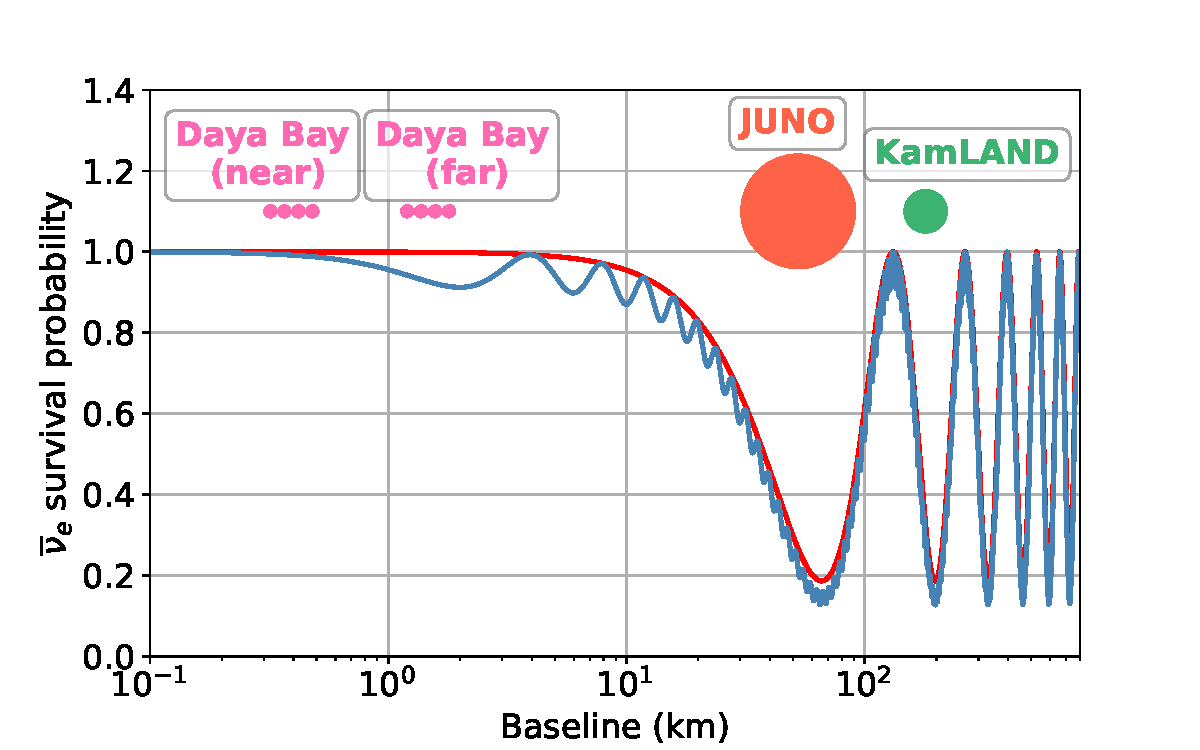
\includegraphics[width=0.9\linewidth]{Img/nuosc_juno.pdf}
\bicaption[反应堆反中微子存活概率随基线的变化]{反应堆反中微子在不同基线下的存活概率。红曲线为由 $\Delta m^2_{21}$ 驱动的慢振荡（太阳项），蓝曲线为包含由 $\Delta m^2_{3\ell}$ 驱动的快振荡在内的三味总存活概率。图中标示了 JUNO（橙色，基线约 52.5\,km，接近太阳振荡极大值）、大亚湾（粉色，近/远基线）和 KamLAND（绿色）的实验基线位置；图片来自文献\citep{abusleme2025measurementreactorneutrinooscillations}}{Reactor $\bar{\nu}_e$ survival probability as a function of baseline for a 4\,MeV antineutrino. The red curve shows the slow (solar) oscillation driven by $\Delta m^2_{21}$, while the blue curve shows the full three-flavor survival probability including the fast (atmospheric) oscillations driven by $\Delta m^2_{3\ell}$. Experimental baselines are indicated for JUNO (orange, 52.5\,km; near the solar-oscillation maximum), Daya Bay (pink, near/far detectors), and KamLAND (green). Taken from Ref\citep{abusleme2025measurementreactorneutrinooscillations}}
\label{fig:reactor_survival_baseline}
\end{figure}

如图~\ref{fig:reactor_survival_baseline} 所示，在不同基线条件下，短基线实验（例如大亚湾近/远站）主要观测由 $\Delta m^2_{31}$/$\Delta m^2_{32}$ 驱动的”快振荡”，其振荡极大值位于约 2\,km 附近；而中长基线实验（例如 JUNO）则位于由 $\Delta m^2_{21}$ 驱动的”慢振荡”极大值附近（约 65\,km），因此 JUNO 能在同一次能谱测量中同时对慢、快两类频率成分敏感。

在传播介质中，中微子除了自由传播相位外，还会与介质中的电子、中子发生相干的前向散射，从而在味基下引入额外的有效势项。对于电子中微子，除中性流外还存在带电流相互作用，产生有效势\cite{Wolfenstein1978,Mikheyev1985}
\begin{equation}
V_e=\sqrt{2}\,G_F N_e,
\label{eq:Ve-matter}
\end{equation}
其中 $G_F$ 为费米常数，$N_e$ 为电子数密度；而缪子与陶子中微子仅有中性流贡献，其在味基下产生的相位相同，可被整体去除。因此在味基下的有效哈密顿量中，电子味分量相对于其它味有一个附加的能量偏移，导致传播本征态（有效质量与有效混合角）偏离真空值。
在两味近似下，可以将物质效应的结果写成对混合角与质量平方差的重整化\cite{Wolfenstein1978Matter, Mikheyev1985Resonance}：
\begin{equation}
\tan(2\theta_m)=\frac{\Delta m^2\sin(2\theta)}
{\Delta m^2\cos(2\theta)-2\sqrt{2}\,G_FN_e E}\,,
\label{eq:tan-2theta-m}
\end{equation}
并且
\begin{equation}
(\Delta m^2_m)^2=\bigl(\Delta m^2\cos2\theta-2\sqrt{2}\,G_FN_eE\bigr)^2
+\bigl(\Delta m^2\sin2\theta\bigr)^2,
\label{eq:dm2m-squared}
\end{equation}
其中 $E$ 为中微子能量，$\theta_m$ 与 $\Delta m^2_m$ 分别为介质中的有效混合角和有效质量平方差。由此可见，当满足共振条件
\begin{equation}
2\sqrt{2}\,G_FN_e E = \Delta m^2\cos(2\theta)
\label{eq:msw-resonance}
\end{equation}
时，$\theta_m$ 接近 $45^\circ$ 并取得极大值——即所谓的 MSW 共振，此时味态转换被显著增强\cite{Mikheyev1985Resonance, Bethe1986Possible}。值得注意的是，共振条件对中微子与反中微子符号相反（因 $V_e$ 对反中微子取负），因此同一介质下中微子与反中微子的物质修正方向不同。

在三味振荡情形中，需对 $3\times3$ 的有效哈密顿量数值对角化以获得精确的物质修正\cite{Zaglauer1988Analytic}；一般而言，物质效应主要影响与太阳项（$\Delta m^2_{21}$）相关的低频分量，而对于快频项（由 $\Delta m^2_{3\ell}$ 驱动）影响较小。对于太阳中微子（穿越太阳高密度区域），MSW 效应产生的大幅增强是解释太阳中微子缺失的关键机制\cite{SNO2002Solar}；而对于穿过地壳传播的反应堆反中微子（基线为数十公里、能量在 MeV 量级），物质势 $V_e$ 的数值通常较小，仅作为微小却必要的修正被纳入精密拟合，以避免在高精度测量（如 JUNO 等）中产生系统偏差\cite{JUNO2016YellowBook, Khan2015Matter}。

\section{江门中微子实验}

JUNO 的首要物理目标是通过精确测量反应堆中微子能谱来确定中微子的质量顺序（正常层级或倒置层级）\cite{An2016_YellowBook}。根据设计，JUNO 在约 6 年运行后可在 $3$--$4\sigma$ 置信度上区分两种质量层级。同时，JUNO 将以亚百分比级的精度精准测量主要振荡参数，如 $\theta_{12}$、$\Delta m^2_{21}$ 和 $\Delta m^2_{31}$，从而进一步完善三味振荡模型\cite{Abusleme2022_Physics}。除反应堆中微子研究外，JUNO 还具备探测太阳中微子、地球（地幔）中微子和超新星中微子的能力，并可进行惰性中微子、质子衰变等新物理现象的探索\cite{An2016_YellowBook}。这些物理目标的实现将为中微子物理学的未来研究提供关键数据和启示。

\subsection{JUNO 的探测器结构与关键参数}

如图\ref{fig:juno_detector}所示，JUNO的核心部件是一个直径35.4米的有机玻璃球形中心探测器，内部装有约20,000吨液体闪烁体\cite{Abusleme2022_Detector}。该玻璃球被浸没在深44米、容积约3.5万吨的水切伦科夫池中，水池既屏蔽周围岩石的本底射线，又安装了光电倍增管作为水切伦科夫探测器，用于标记通过的宇宙射线μ子\cite{Abusleme2025}。中心有机玻璃球外壁均匀布置了约20000只20英寸光电倍增管和25600只3英寸光电倍增管，用于收集来自闪烁体的光信号，这一双量能器系统（Dual-calorimetry）能够有效提升动态范围与校准精度\cite{Abusleme2022_PMT}。为了进一步抑制宇宙μ子背景，在水池顶部还安装有塑料闪烁体顶层径迹探测器（Top Tracker），用于精确记录穿过探测器的μ子轨迹并作为μ子标记\cite{Grassmann2014_TT}。

\begin{figure}[htbp]
    \centering
    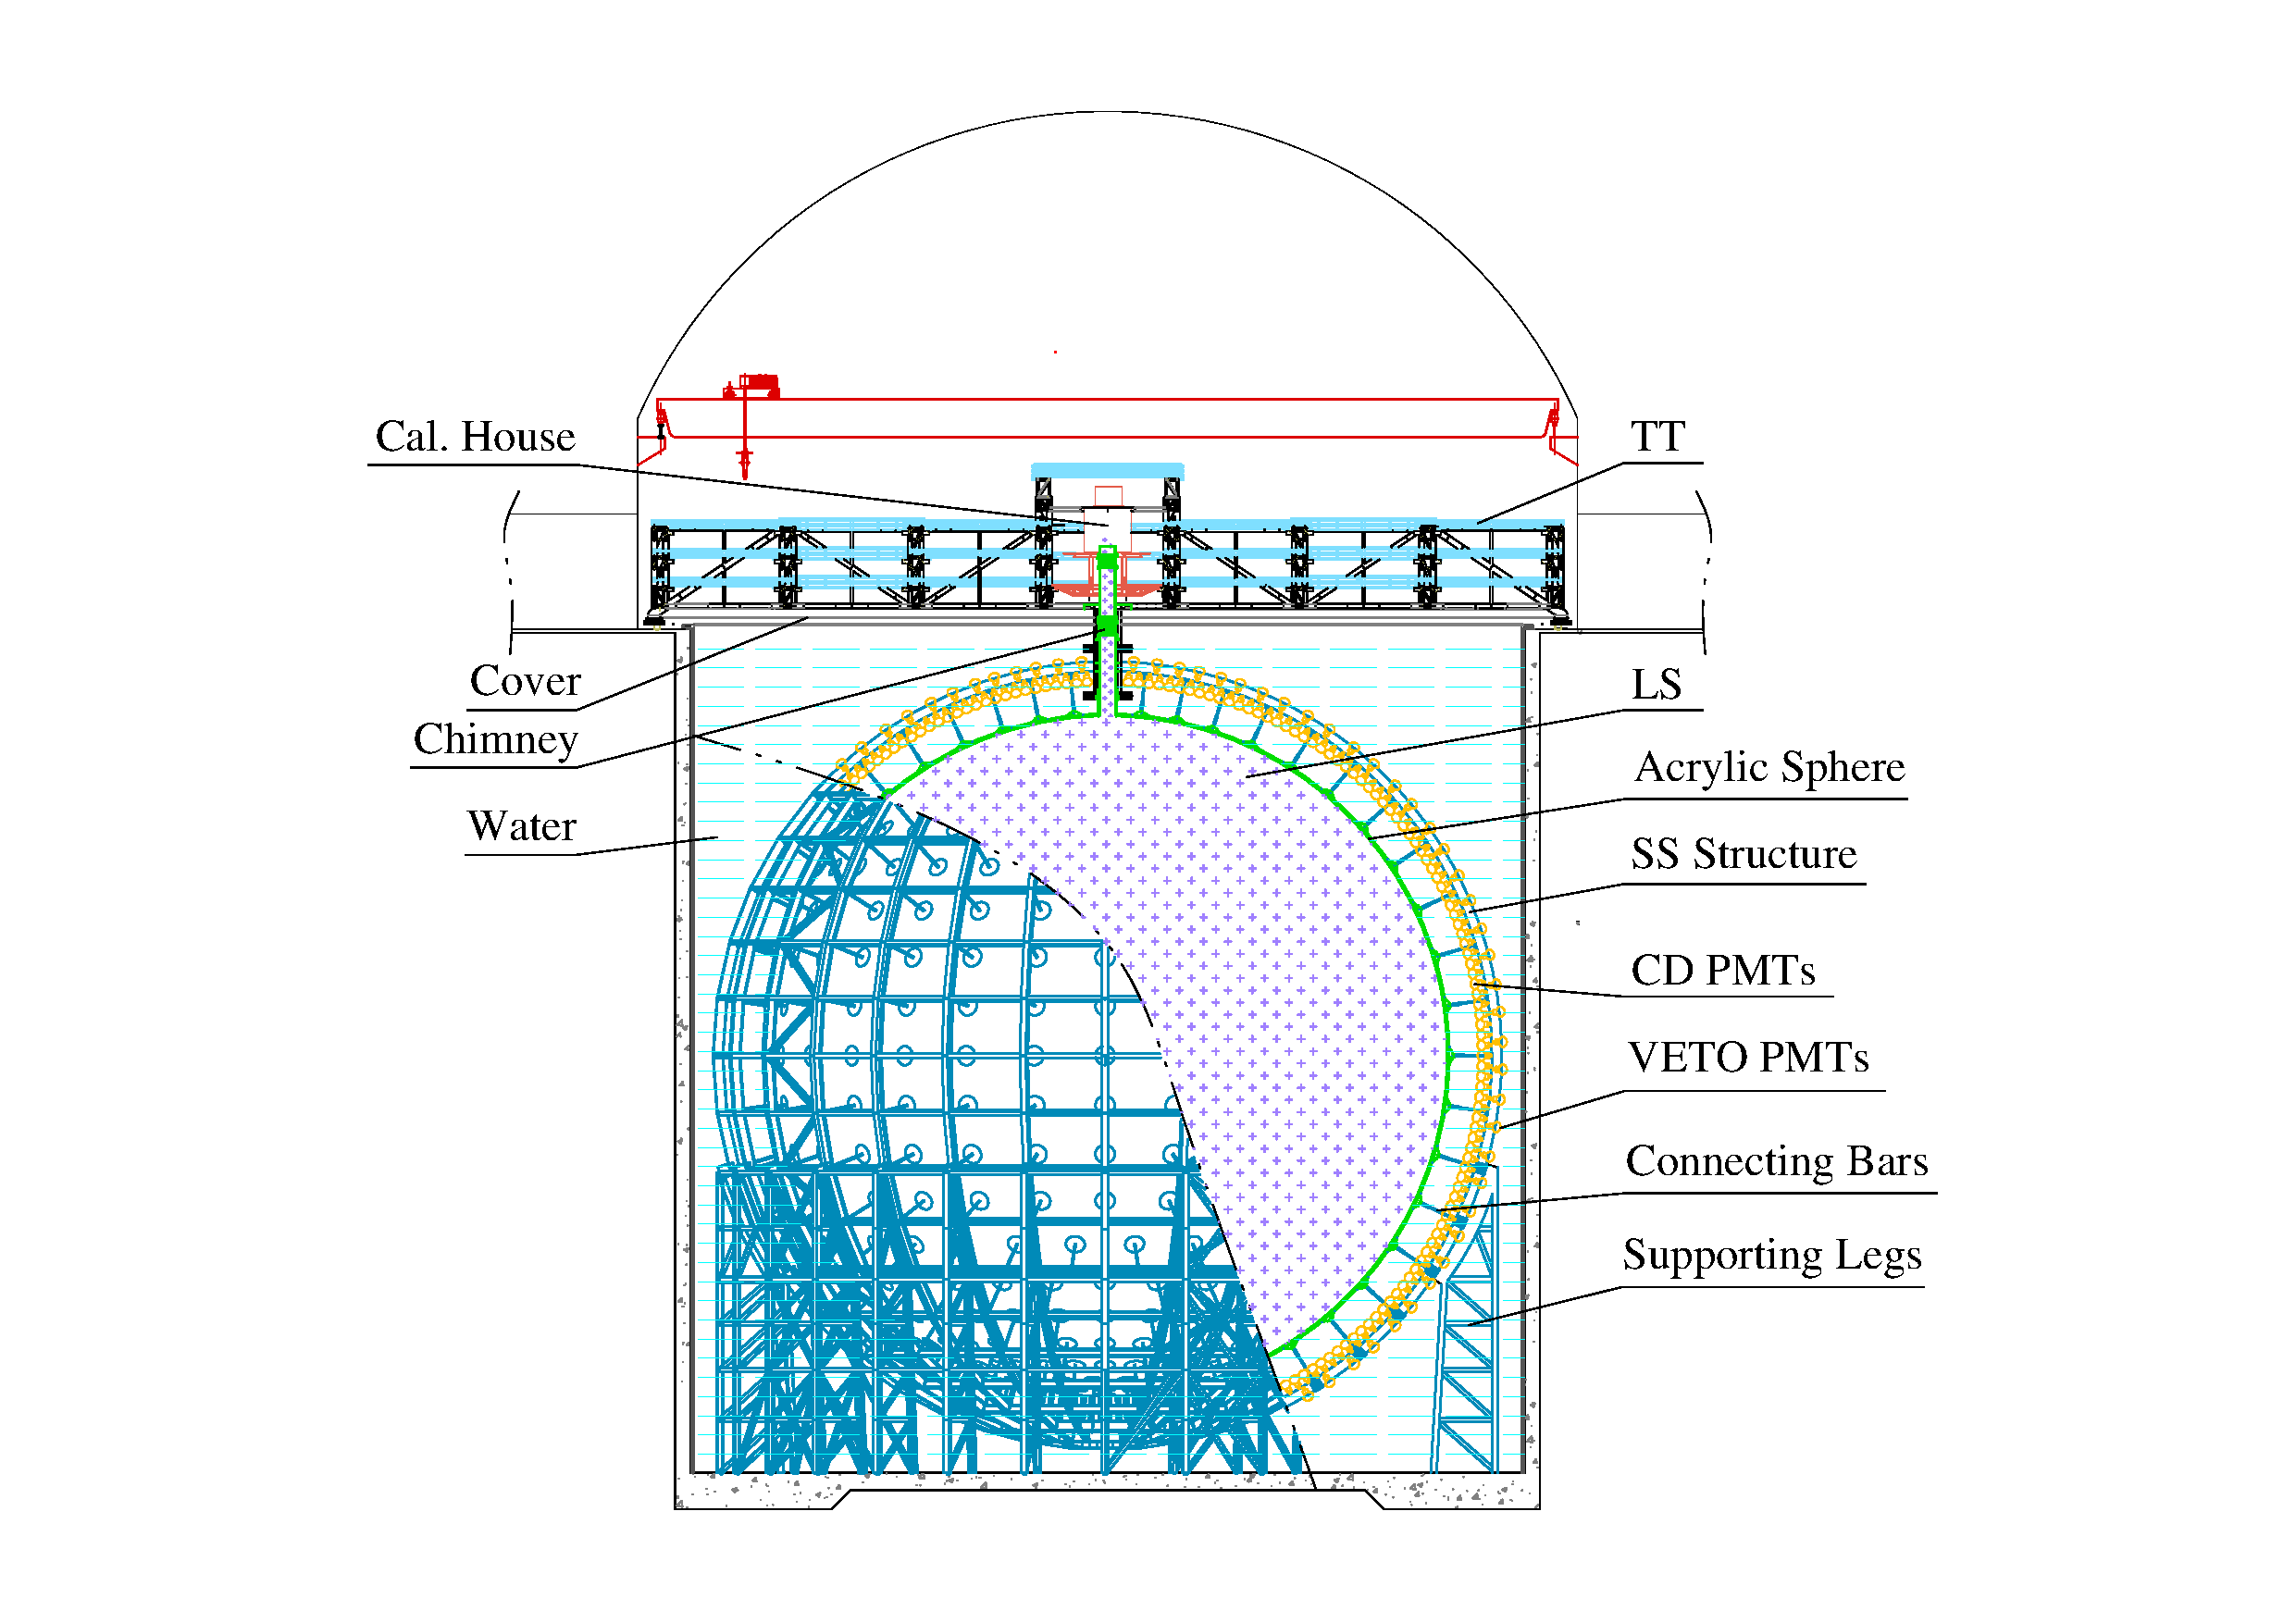
\includegraphics[width=0.9\linewidth]{Img/JUNO_Detector_Scheme.pdf}
    \bicaption[JUNO 探测器示意图]{JUNO 探测器示意图（图片来自文献\cite{Abusleme2025}）。}{Schematic view of the JUNO detector, taken from Ref.\cite{Abusleme2025}.}
    \label{fig:juno_detector}
\end{figure}

JUNO 探测器的关键指标之一是极高的能量分辨率。设计要求在 1~MeV 处达到约 3\% 的能量分辨率，相当于每 MeV 产生超过 1100 个探测光电子\cite{Abusleme2021_LS}。为此，探测器选用了高透射性的 LAB 基液体闪烁体，掺有荧光体 PPO 和波长转换剂 Bis-MSB\cite{Abusleme2021_LS}。探测器中安装了约 20000 只 20 英寸高效 PMT 和 25600 只 3 英寸 PMT，光电覆盖率约为 75\%，保证了足够的光收集效率以实现上述能量分辨率目标\cite{Abusleme2022_PMT}。

\subsection{JUNO 中的反应堆中微子}
JUNO 协作组于 2025 年底发布了首篇反应堆中微子振荡物理结果论文《First measurement of reactor neutrino oscillations at JUNO》\citep{abusleme2025measurementreactorneutrinooscillations}。该结果基于探测器完工后自 2025 年 8 月以来的 59.1 天数据，共选取到 2379 个逆 $\beta$ 衰变（IBD）中微子候选事件。通过对中微子快信号能谱的拟合分析，得到了真空三味振荡参数的高精度测量结果。

\begin{figure}[htbp]
\centering
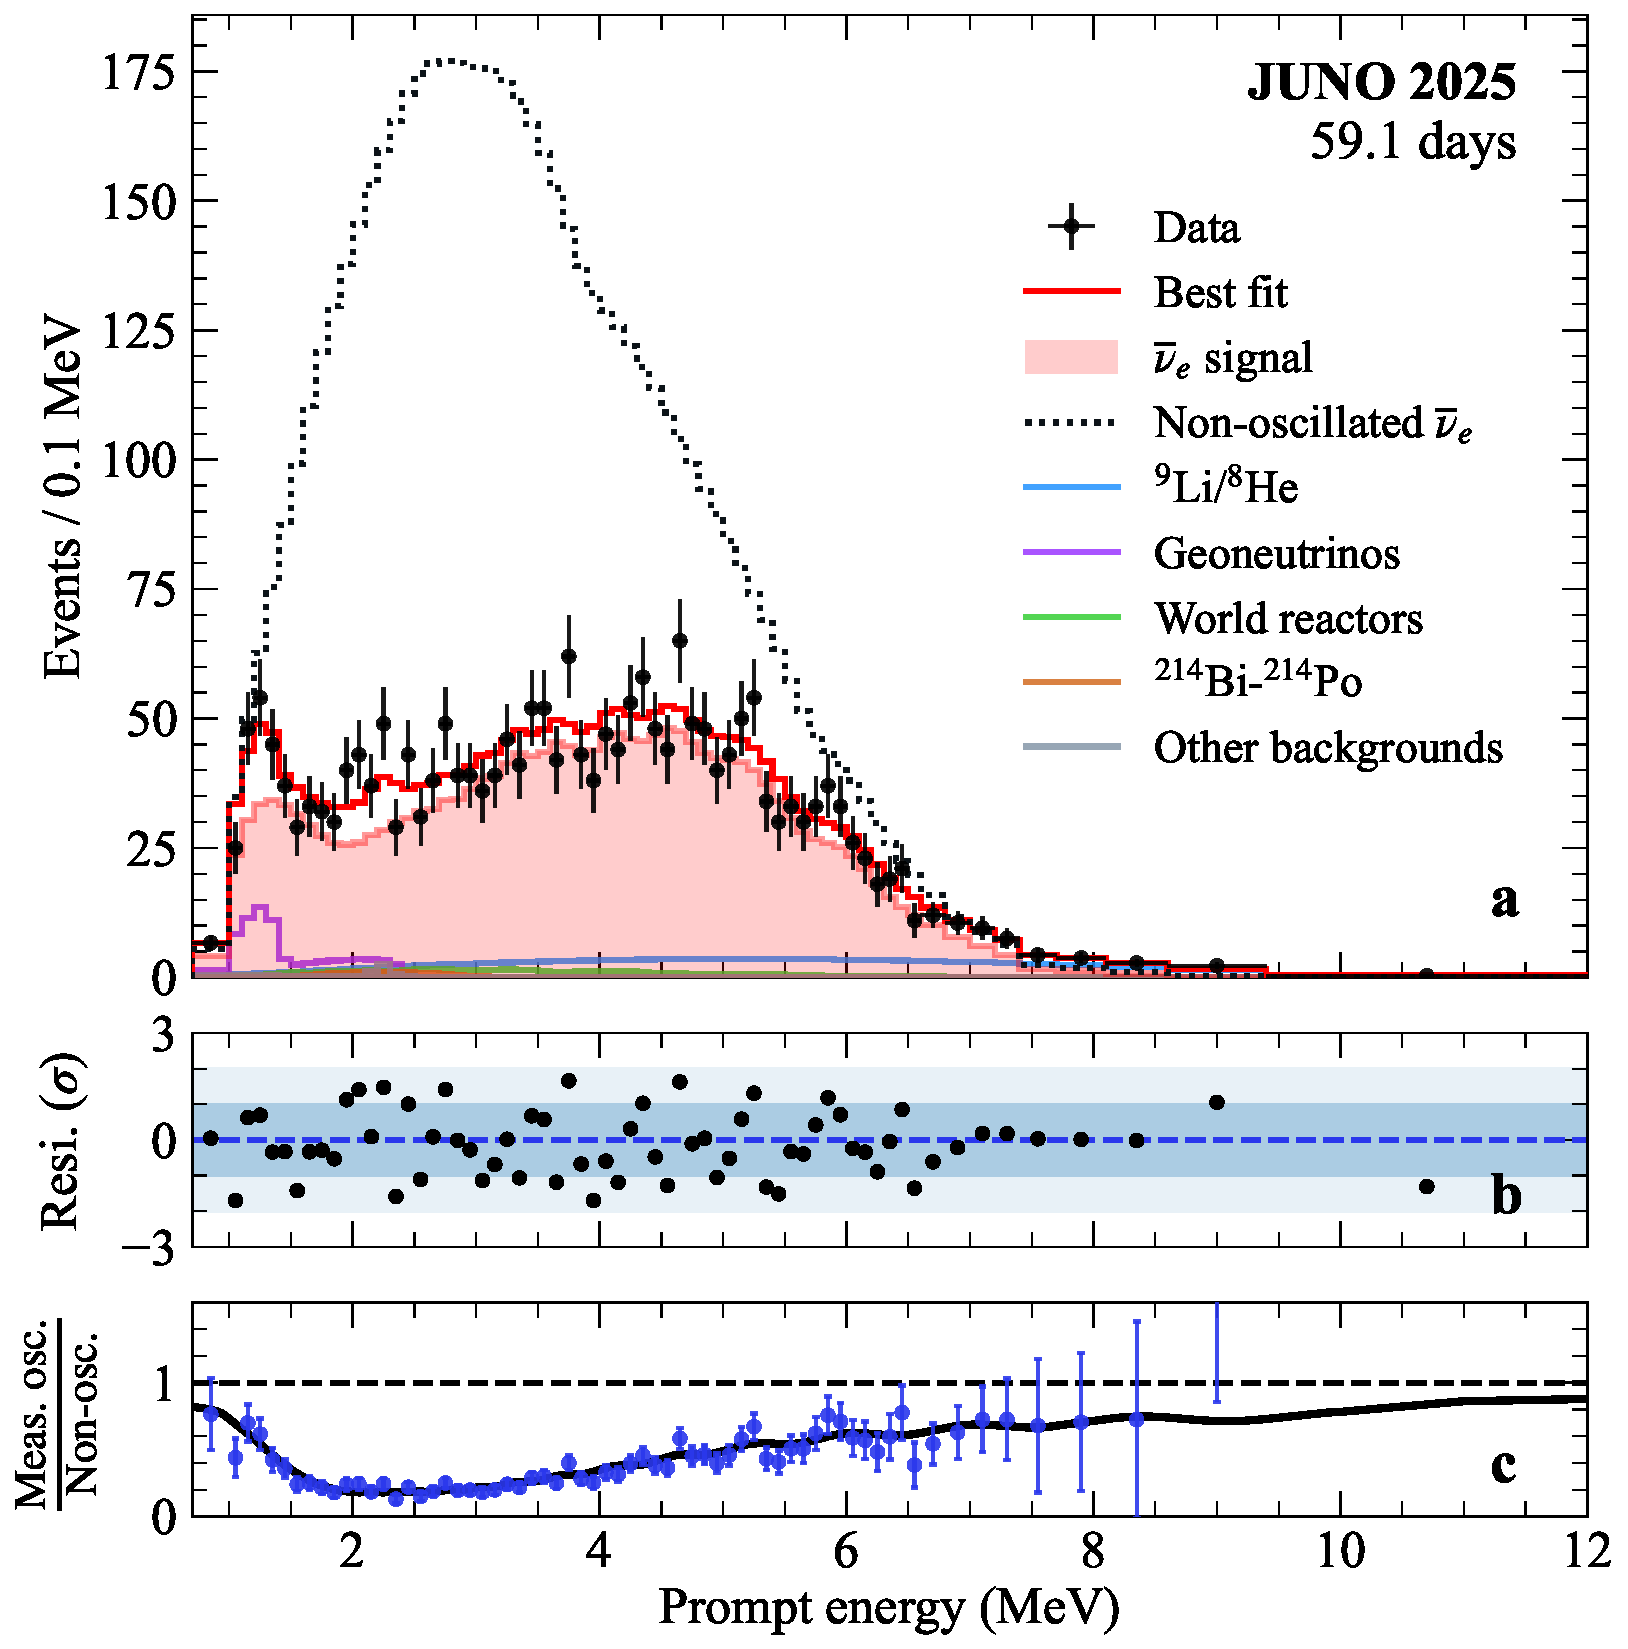
\includegraphics[width=0.9\linewidth]{Img/antineutrinoSpectrum.pdf}
\bicaption[测量能谱及拟合结果（JUNO 首篇物理分析结果，59.1 天数据）]{（a）黑点为经过事例挑选后的IBD 候选事例的测量值（带统计误差），红色实线为包含振荡效应的最佳拟合模型，红色阴影区为拟合出的反中微子信号分量。黑色虚线为若无振荡时的反应堆中微子预期谱。其他有色实线分别表示主要本底成分（例如宇宙线次级粒子$^9$Li/$^8$He、地球中微子、来自全球反应堆的中微子贡献、$^{214}$Bi--$^{214}$Po 等）。（b）数据与完整模型之间的残差及其一致性检验。（c）测得的振荡后谱与无振荡预测之比，显示能谱上的振荡形状特征。该图直接展示了在短期运行下 JUNO 对 IBD 能谱的重建能力与振荡信号的显著性（见文献\cite{abusleme2025measurementreactorneutrinooscillations}）。}{Prompt IBD energy spectrum and fit results (JUNO first physics measurement, 59.1 days). (a) Black points show the measured prompt energy distribution of selected IBD candidates with statistical error bars. The red curve indicates the best-fit oscillation model and the red shaded band denotes the fitted antineutrino signal component. The black dotted curve illustrates the non-oscillated reactor antineutrino expectation. Colored solid lines indicate major background contributions (e.g.\ cosmogenic $^9$Li/$^8$He, geoneutrinos, distant reactor background, $^{214}$Bi--$^{214}$Po, etc.). (b) Residuals quantifying the statistical consistency between data and the full model (in units of $\sigma$). (c) Ratio of the measured oscillated spectrum to the non-oscillated prediction, highlighting the spectral distortions induced by neutrino oscillations. Data are from JUNO Collaboration, First measurement of reactor neutrino oscillations at JUNO (59.1 days)\cite{abusleme2025measurementreactorneutrinooscillations}.}
\label{fig:juno_prompt_spectrum}
\end{figure}

图~\ref{fig:juno_prompt_spectrum} 展示了 JUNO 在首个 59.1 天采集期内的测量能谱、振荡最佳拟合与各类本底构成：测量谱与无振荡预测存在显著偏离，且谱形的能量依赖失真与三味振荡模型的拟合结果高度一致，直观证明了 JUNO 在能谱学测量和振荡参数约束上的能力。在假定正常质量序的情况下，测得 $\sin^2\theta_{12}=0.3092\pm0.0087$ 和 $\Delta m^2_{21}=(7.50\pm0.12)\times10^{-5}\,\mathrm{eV}^2$。

\begin{figure}[htbp]
\centering
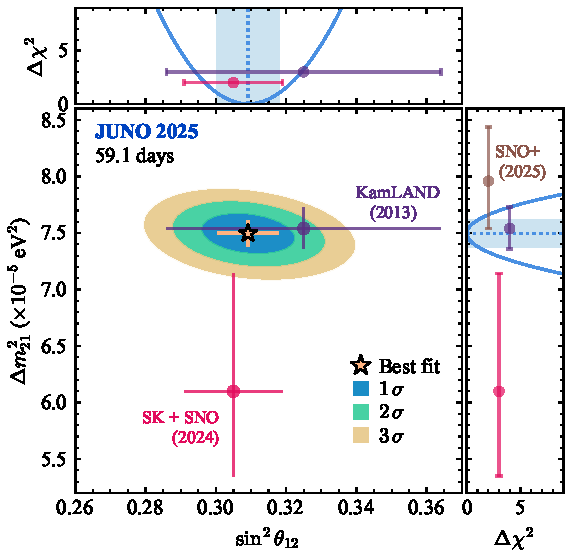
\includegraphics[width=0.9\linewidth]{Img/contour_sinsq12_dmsq21_withOtherExp.pdf}
\bicaption[太阳振荡参数约束（JUNO 59.1 天数据）]{基于 2025 年 59.1 天 JUNO 数据，通过对反应堆反中微子快信号能谱进行谱拟合得到的太阳振荡参数 $\sin^2\theta_{12}$ 与 $\Delta m_{21}^2$ 的约束结果。阴影椭圆区域分别对应 $1\sigma$、$2\sigma$ 和 $3\sigma$ 置信区间。上方（右侧）面板给出了对另一参数进行 profile 处理后得到的 $\sin^2\theta_{12}$（$\Delta m_{21}^2$）的一维 $\Delta\chi^2$ 分布。星号表示 JUNO 的最佳拟合值，误差棒表示对应的一维 $1\sigma$ 置信区间。同时给出了 KamLAND (2013)、SNO+ (2025) 以及 Super-Kamiokande 与 SNO 联合分析 (2024) 的结果以作比较。（见文献\cite{abusleme2025measurementreactorneutrinooscillations}）}{Constraints on the solar oscillation parameters $\sin^2\theta_{12}$ and $\Delta m_{21}^2$ obtained from a spectral fit to the measured prompt energy spectrum of reactor antineutrinos with 59.1 days of JUNO data (2025). The shaded elliptical regions correspond to the $1\sigma$, $2\sigma$, and $3\sigma$ confidence levels. The upper (right) panel shows the one-dimensional $\Delta\chi^2$ profile for $\sin^2\theta_{12}$ ($\Delta m_{21}^2$), where the other parameter is profiled. The star denotes the JUNO best-fit point, and the error bars indicate the corresponding $1\sigma$ intervals. Results from KamLAND (2013), SNO+ (2025), and the combined Super-Kamiokande (SK) + SNO (2024) analyses are shown for comparison.\cite{abusleme2025measurementreactorneutrinooscillations}}
\label{fig:juno_contour}
\end{figure}

图~\ref{fig:juno_contour} 表明这一测量精度比以往实验的组合结果提高了约 1.6 倍。JUNO 已能够通过反应堆反中微子能谱的精密测量，对太阳振荡参数 $\sin^2\theta_{12}$ 和 $\Delta m_{21}^2$ 给出具有竞争力的独立约束。系统误差方面，通过大量校准保证了能量标度不确定度约 $0.5\%$、正电子非线性约 $1\%$ 的约束；同时对来自宇宙射线次级粒子 $^9$Li/$^8$He 衰变等本底进行了严格抑制。实验结果为未来利用 JUNO 数据精确探究中微子质量顺序奠定了良好基础。

\subsection{JUNO 中的大气中微子}
JUNO 探测器还可观测大气中微子，其能量范围从100 MeV 到 10 GeV\citep{Abusleme2021}，通道覆盖从近地表至地球直径的路径长度（最长约 $1.3\times10^4\,\mathrm{km}$），对应广泛的 $L/E$ 范围（从几百到上万 km/GeV）。在几 GeV 以上能量区间内，JUNO 具有良好的能量和角分辨能力：对于 $E_\nu>3\,\mathrm{GeV}$ 的电子型大气中微子，能量重建优于 $6\%$，缪子型优于 $8\%$；其到达方向的角度分辨率在 $\sim10^\circ$ 量级。这些精度使 JUNO 能够通过对大气中微子在地球介质中出现的 MSW 效应进行研究，从而补充其主要的质量序测定方案。目前 JUNO 尚未发布大气中微子观测结果，但相关研究表明，利用大约 10 年的数据，大气中微子通道可提供约 $1.0$--$1.8\sigma$ 的质量序敏感度\citep{Zhang2023OscillationPhysicsPotential}。特别是将大气中微子结果与反应堆中微子结果结合分析，有望进一步增强整体灵敏度。

\begin{figure}[htbp]
\centering
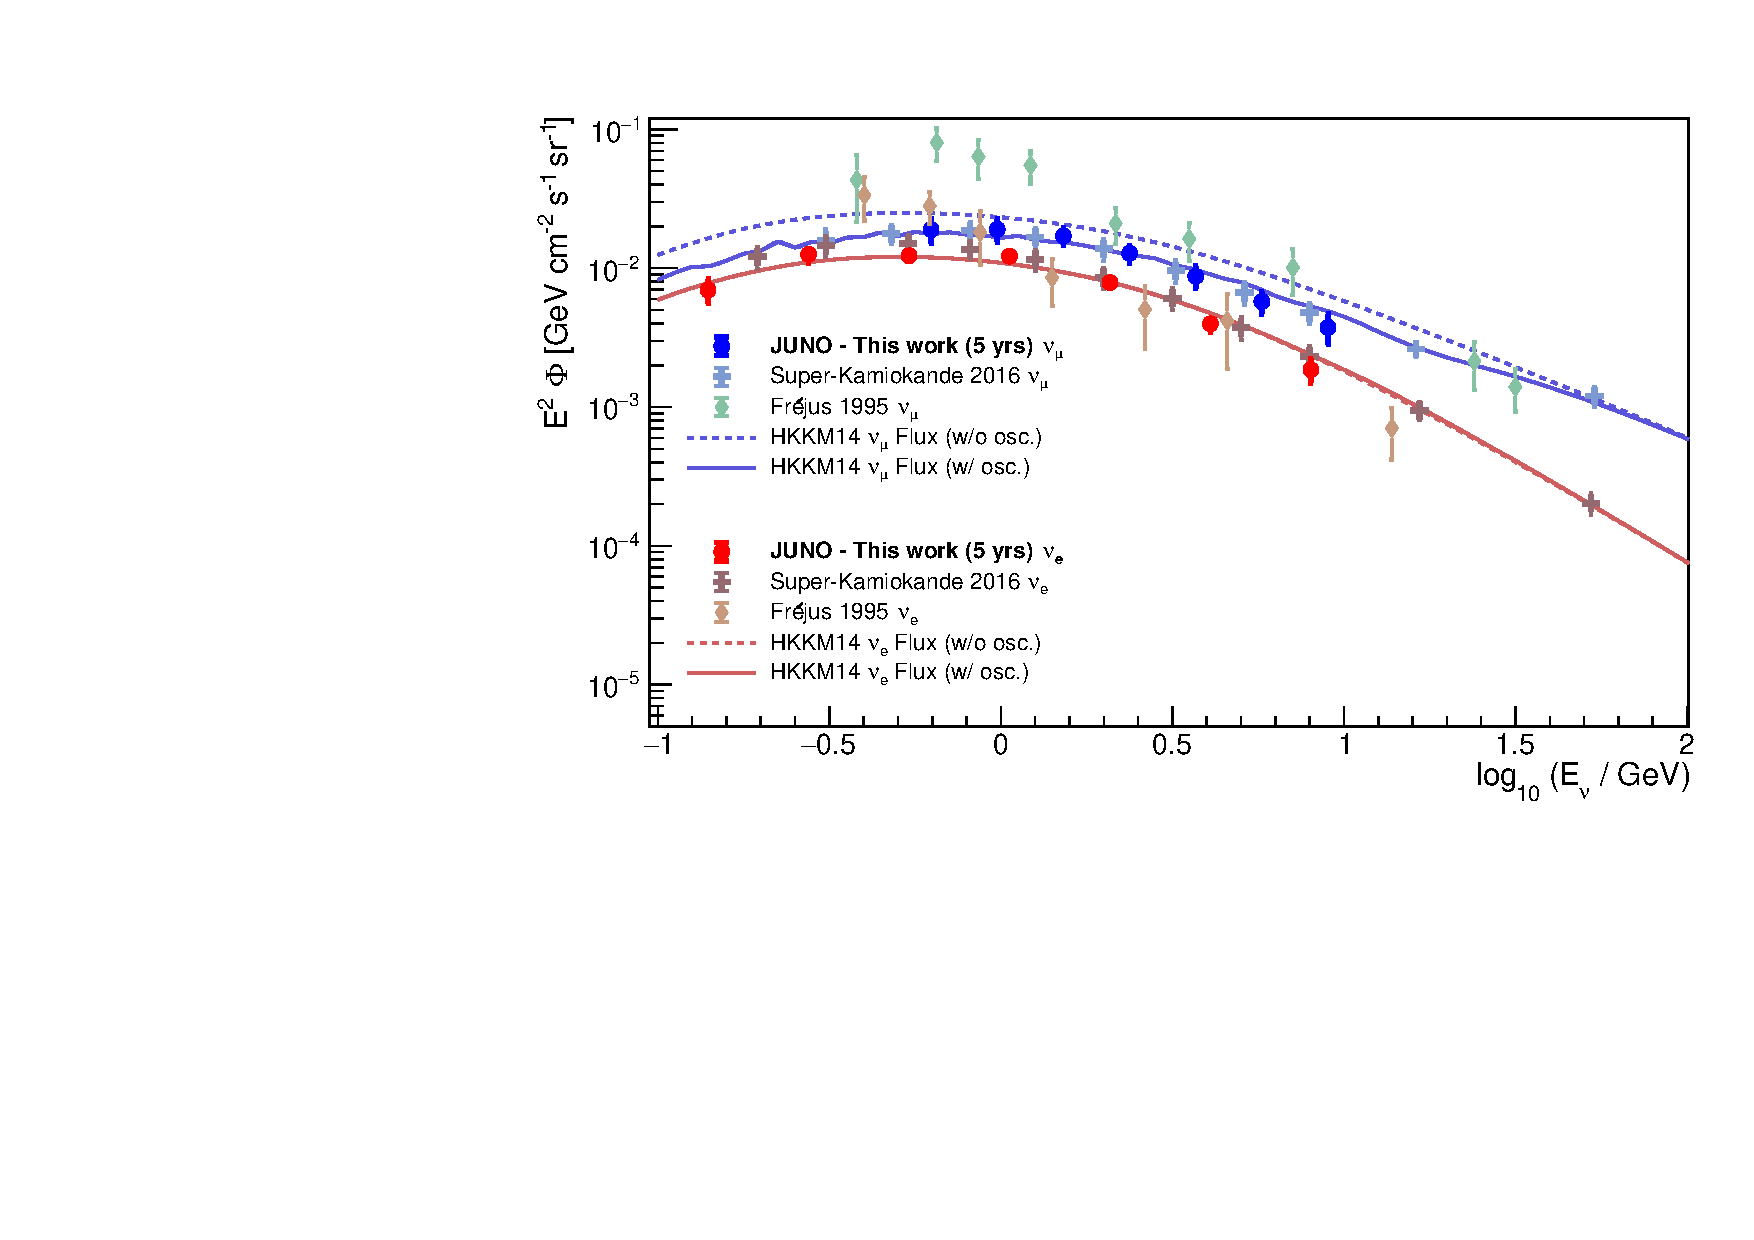
\includegraphics[width=0.9\linewidth]{Img/AtmoSpec_ALL_YB.pdf}
\bicaption[JUNO 对大气中微子能谱的灵敏度预期与现有实验结果比较]{JUNO 对大气中微子能谱的灵敏度预期与现有实验结果比较。图中给出了在 5 年运行时间下，JUNO 对大气中微子通量 $E^2\Phi$ 的预期测量结果（蓝色为 $\nu_\mu$，红色为 $\nu_e$），并与 Super-Kamiokande 2016 年测量结果以及 Fréjus 1995 年数据进行比较。同时给出了 Honda--Kajita--Kasahara--Midorikawa（HKKM14）大气中微子通量模型在考虑振荡（实线）和不考虑振荡（虚线）情况下的理论预期。横轴为中微子能量的对数刻度 $\log_{10}(E_\nu/\mathrm{GeV})$，纵轴为 $E^2\Phi$。可以看出，在 GeV 能区，振荡效应对 $\nu_\mu$ 通量产生显著压低，而 $\nu_e$ 通量则表现出相对增强或形状变化。JUNO 的测量精度在多 GeV 区间内具有良好的统计灵敏度，可用于检验大气中微子振荡模型并辅助质量顺序分析。该图来自文献\citep{Abusleme2025}}{Expected JUNO sensitivity to atmospheric neutrino flux compared with previous measurements and theoretical predictions. The figure shows the projected 5-year JUNO measurement of the atmospheric neutrino flux in terms of $E^2\Phi$ (blue points for $\nu_\mu$, red points for $\nu_e$). The results are compared with Super-Kamiokande 2016 measurements and Fréjus 1995 data. Theoretical predictions from the HKKM14 atmospheric neutrino flux model are shown both without oscillation (dashed lines) and with oscillation (solid lines). The horizontal axis represents $\log_{10}(E_\nu/\mathrm{GeV})$, and the vertical axis corresponds to $E^2\Phi$. The figure illustrates the suppression of $\nu_\mu$ flux due to oscillation effects in the GeV region, while modifications in the $\nu_e$ spectrum are also visible. JUNO demonstrates competitive sensitivity in the multi-GeV range, enabling further tests of atmospheric neutrino oscillations and complementary constraints on the neutrino mass ordering. Taken from Ref\citep{Abusleme2025}}
\label{fig:atmos_nu}
\end{figure}

如图~\ref{fig:atmos_nu} 所示，在 5 年运行时间下，JUNO 对 GeV 能区大气中微子通量的测量预期与 HKKM14 理论模型符合良好，并能够清晰分辨振荡与非振荡情形的差异，从而为质量顺序判定提供独立而互补的实验信息。

\subsection{JUNO 中的太阳中微子}
标准太阳模型预言太阳中微子主要来源于 pp 链和 CNO 循环反应，其能谱分布如图~\ref{fig:solar_nu_spectrum} 所示。

\begin{figure}[htbp]
\centering
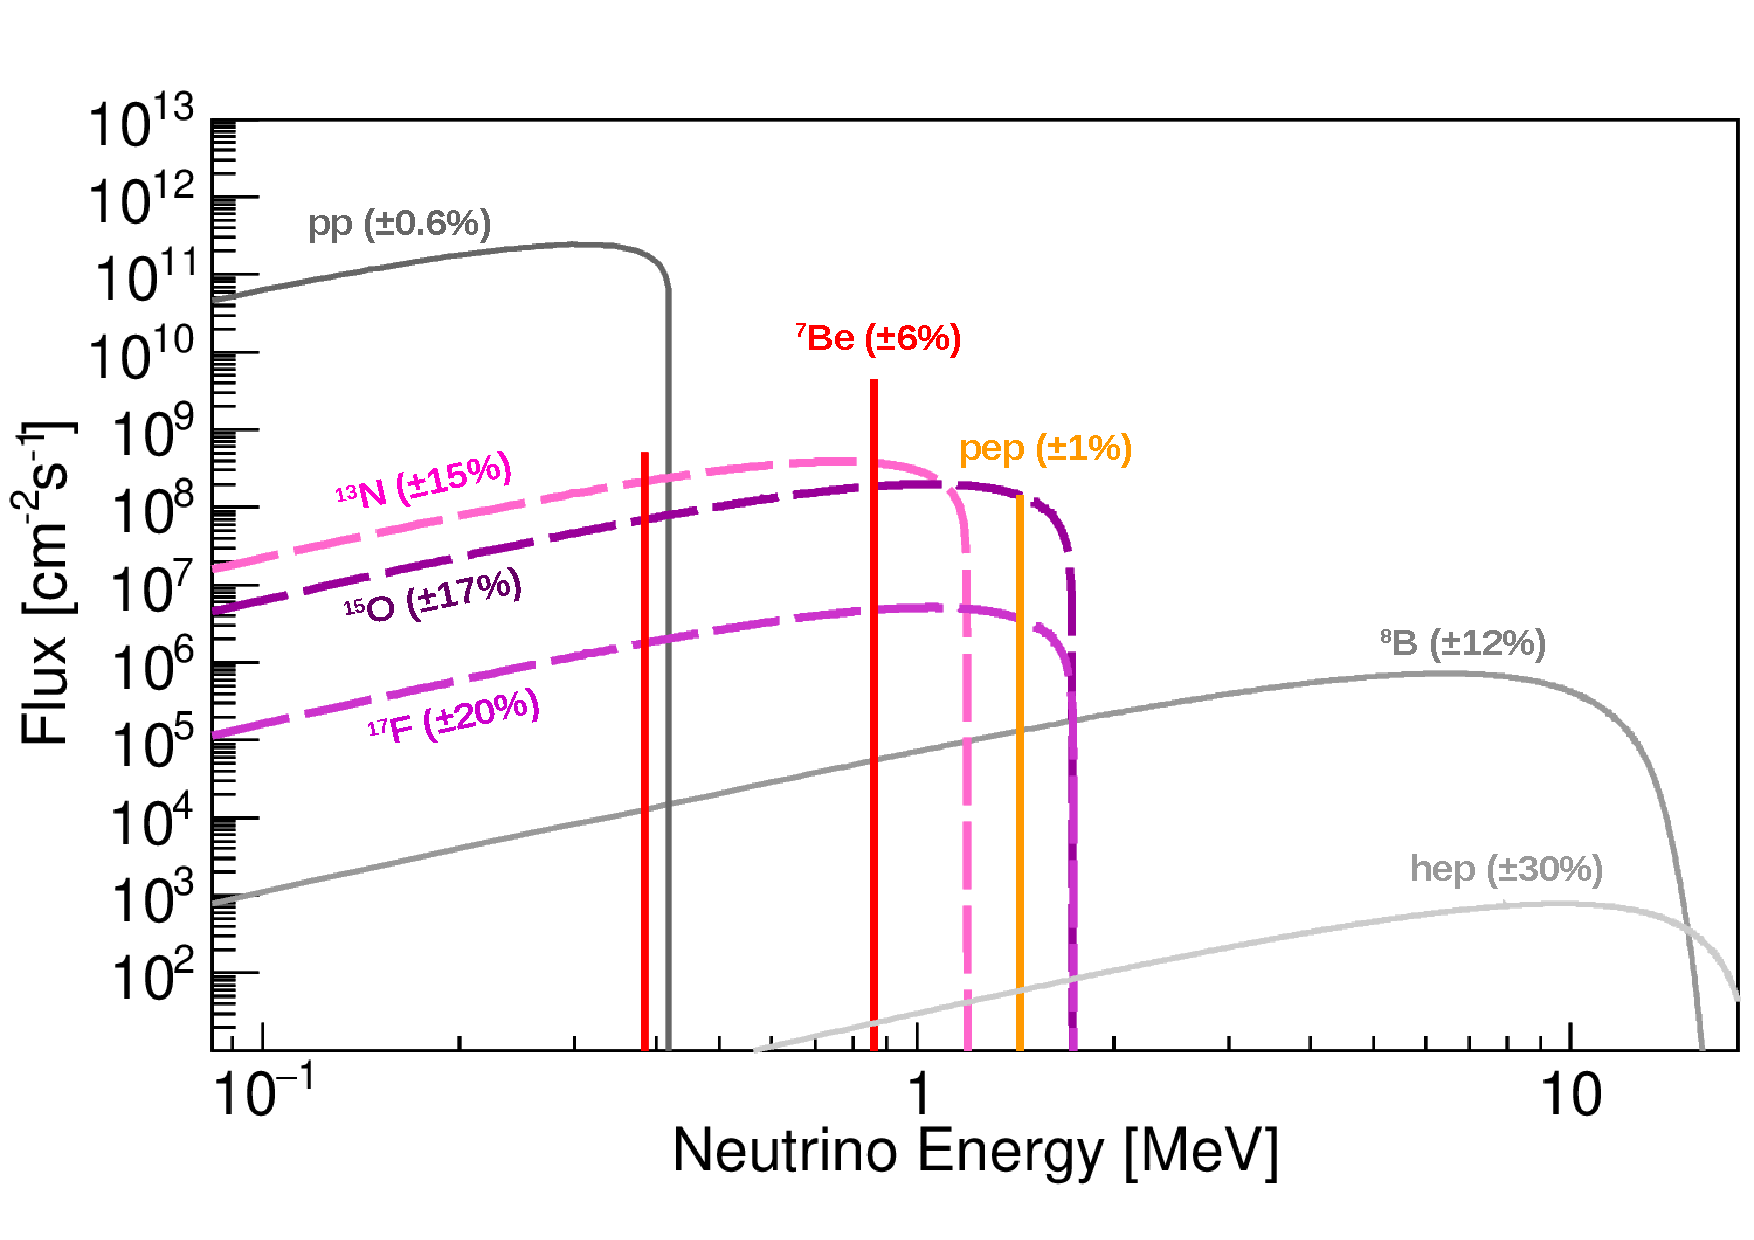
\includegraphics[width=0.9\linewidth]{Img/Fig2_v5.pdf}
\bicaption[太阳中微子能谱及理论通量预测]{太阳中微子能谱及理论通量预测。图中给出了标准太阳模型（Standard Solar Model, SSM）预测的各类太阳中微子通量随能量变化关系，包括 pp、$^7$Be、pep、$^8$B、hep 以及 CNO 循环产生的 $^{13}$N、$^{15}$O、$^{17}$F 中微子。不同曲线对应不同反应来源，括号中标注为理论通量的不确定度。红色和橙色竖线分别标示了 JUNO 对 $^7$Be 和 pep 单能谱太阳中微子的主要灵敏能区。该图展示了低能 pp 与 $^7$Be 中微子在太阳中微子总通量中的主导地位，以及高能 $^8$B 与 hep 中微子在高能区的重要贡献。图片来自文献\citep{Abusleme_2023}}{Solar neutrino fluxes predicted by the Standard Solar Model (SSM). The figure shows the theoretical solar neutrino flux as a function of neutrino energy for different components, including pp, $^7$Be, pep, $^8$B, hep, and CNO-cycle neutrinos ($^{13}$N, $^{15}$O, $^{17}$F). The quoted percentages indicate the theoretical uncertainties of each flux component. The red and orange vertical lines indicate the primary sensitivity regions of JUNO for monoenergetic $^7$Be and pep neutrinos. The figure highlights the dominance of pp and $^7$Be neutrinos in the low-energy region and the contribution of $^8$B and hep neutrinos at higher energies.Taken from Ref\citep{Abusleme_2023}}
\label{fig:solar_nu_spectrum}
\end{figure}

低能区（$E_\nu<2\,\mathrm{MeV}$）主要由 pp、$^7$Be 和 pep 中微子主导，其中 $^7$Be 为单能谱中微子，在约 $0.86\,\mathrm{MeV}$ 处形成明显特征信号；而高能区则由 $^8$B 与 hep 中微子贡献。JUNO 由于具有大体积液体闪烁体和优异的能量分辨率（约 $3\%$ @ $1\,\mathrm{MeV}$），在抑制放射性本底后，有望实现对 $^7$Be（$862\,\mathrm{keV}$）、pep（$1.44\,\mathrm{MeV}$）和 CNO 循环（$1$--$2\,\mathrm{MeV}$）中微子的精确测量，从而进一步检验太阳模型并研究低能区的物质增强振荡效应（MSW-LMA 区域）。研究表明，在达到与 Borexino 相当的极低本底放射纯度水平时，JUNO 有望在绝大多数情况下优于现有对这三种中微子通量的精密测量\citep{Abusleme_2023}。目前 Borexino 已分别以 $2.7\%$ 精度测出 $^7$Be 中微子通量，并首次 $5\sigma$ 检出 pep 中微子和 CNO 中微子的存在，但其探测器规模仅 100 吨量级。相比之下，JUNO 拥有 20 千吨的大体积液体闪烁体，统计灵敏度显著更高；但要实现同样水平的本底抑制，需要将 $^{238}$U、$^{232}$Th 及 $^{210}$Bi/$^{210}$Po 等内在放射性控制到极低水平。若材料纯化和屏蔽达标，模拟表明 JUNO 可在 1 年内记录上百至数百个 $^7$Be/pep 事件，并在 CNO 中微子通量的测量上取得突破\citep{Abusleme_2023}。JUNO 对太阳中微子的系统亮点在于大体积带来的统计优势和极高能量分辨，但挑战在于非信号本底（如 $^{85}$Kr、$^{11}$C 等）的控制。因此，JUNO 将重点优化极低本底条件下的事例挑选和能谱拟合方法，以期达到或超越 Borexino 在 ppm 级别本底控制的灵敏度。



\subsection{JUNO 中的超新星中微子}
JUNO 对银河系内超新星的中微子爆发具极强响应能力。根据模型预估，一场典型的核心塌缩超新星爆发将在约 10 秒内产生大量低能中微子信号：IBD 通道（$\bar\nu_e+p\to e^++n$）可记录约 5000 个事件，弹性散射通道（中微子与电子散射）记录约 300 个事件，而中微子与质子散射通道可记录 $\sim2000$ 个事件\citep{Lombardo2023SupernovaJUNO}。

\begin{figure}[htbp]
\centering
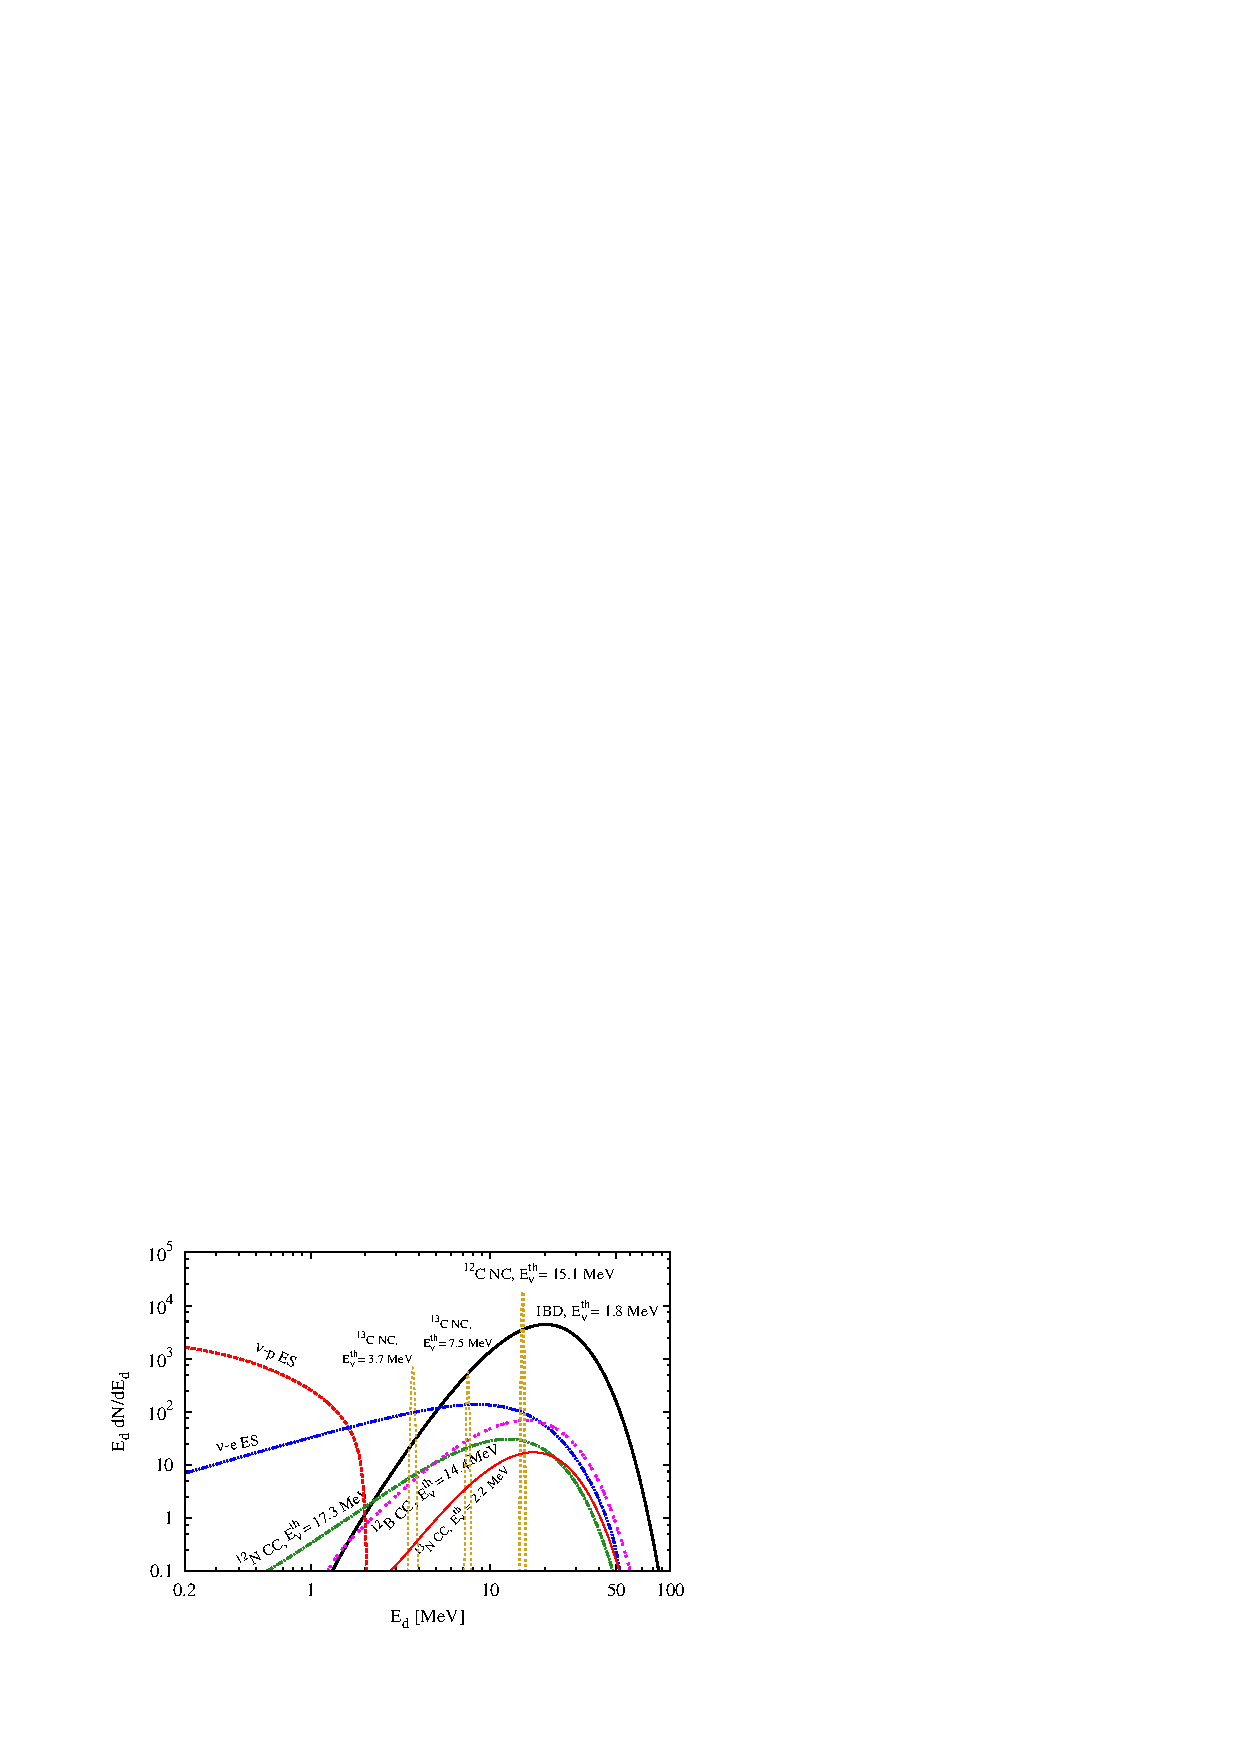
\includegraphics[width=0.9\linewidth]{Img/SNspectra.pdf}
\bicaption[JUNO 探测器中不同超新星中微子相互作用通道的沉积能量分布]{JUNO 探测器中不同超新星中微子相互作用通道的沉积能量分布。图中给出了在一次典型银河系核心坍缩超新星爆发条件下，JUNO 探测器内不同反应通道的可观测沉积能量 $E_{\mathrm{d}}$ 分布，包括反 $\beta$ 衰变（IBD，$\bar{\nu}_e + p \to e^+ + n$）、电子弹性散射（$\nu$--e ES）、质子弹性散射（$\nu$--p ES）、以及在 $^{12}$C 和 $^{13}$C 上的带电流（CC）与中性流（NC）反应。图中同时标注了各反应的能量阈值 $E_\nu^{\mathrm{th}}$。可以看到，IBD 通道在数十 MeV 能区贡献最大，是 JUNO 探测超新星 $\bar{\nu}_e$ 的主导通道；图片来自文献\citep{Abusleme2025}}{Deposited energy distributions of different supernova neutrino interaction channels in JUNO. The figure shows the visible deposited energy $E_{\mathrm{d}}$ spectra in JUNO for various interaction channels induced by a typical core-collapse supernova neutrino burst. These include inverse beta decay (IBD, $\bar{\nu}_e + p \to e^+ + n$), neutrino--electron elastic scattering ($\nu$--e ES), neutrino--proton elastic scattering ($\nu$--p ES), and charged-current (CC) and neutral-current (NC) interactions on $^{12}$C and $^{13}$C. The neutrino energy thresholds $E_\nu^{\mathrm{th}}$ for each reaction are indicated. The IBD channel dominates in the tens-of-MeV region and provides JUNO's primary sensitivity to $\bar{\nu}_e$. Taken from Ref\citep{Abusleme2025}}
\label{fig:supernova_channels}
\end{figure}

如图~\ref{fig:supernova_channels} 所示，反 $\beta$ 衰变通道在数十 MeV 能区具有最高统计量，是 JUNO 探测超新星 $\bar{\nu}_e$ 的核心通道；同时，$^{12}$C 与 $^{13}$C 上的中性流反应以及弹性散射通道为研究全味道中微子谱及爆发动力学过程提供了重要补充信息。此外，中微子与碳原子核的相互作用（含带电流和中性流反应）也会贡献数百个事件。如此高的统计量可让 JUNO 对超新星信号进行时域和能谱的精细测量，检验超新星核心坍缩模型\citep{Li2020Prospects}。JUNO 探测器还可参与国际超新星预警网络（SNEWS），在探测到信号时提供爆发的预警定位。研究估计，当观测到约 5000 个 IBD 事件时，JUNO 对超新星方向的定位精度可达到约 $9^\circ$ 不确定度\citep{Lorenz2016NeutrinoAstroJUNO}，足以配合光学望远镜迅速搜索可能的爆发源。

\subsection{JUNO 中的地球中微子}
JUNO 设计同样适用于探测来自地球内部放射性元素衰变产生的地球中微子（主要来源于 $^{238}$U 和 $^{232}$Th 衰变链）。利用与反应堆中微子相同的 IBD 反应，JUNO 每年预计可记录约 400 个地球中微子事件\citep{Ludhova2023JUNOStatus}。这一统计量远超当前 Borexino 和神冈两个实验多年来的累计结果（Borexino 约 50 个/年，神冈约 100 个/年）。如此高的事件率意味着 JUNO 将很快达到现有实验的灵敏度，并进一步精确测定地球中微子通量\citep{Ludhova2023JUNOStatus}。地球中微子的测量在地质学上意义重大：它为估算地幔与岩石圈中放射性元素丰度提供了独一无二的探针，可进一步推算地球的放射生热总量。JUNO 的测量还可以对 $^{232}$Th/$^{238}$U 比值进行约束，从而帮助验证地球化学模型对深部地热源贡献的预测\citep{Li2026Prospects}。

\begin{figure}[htbp]
\centering
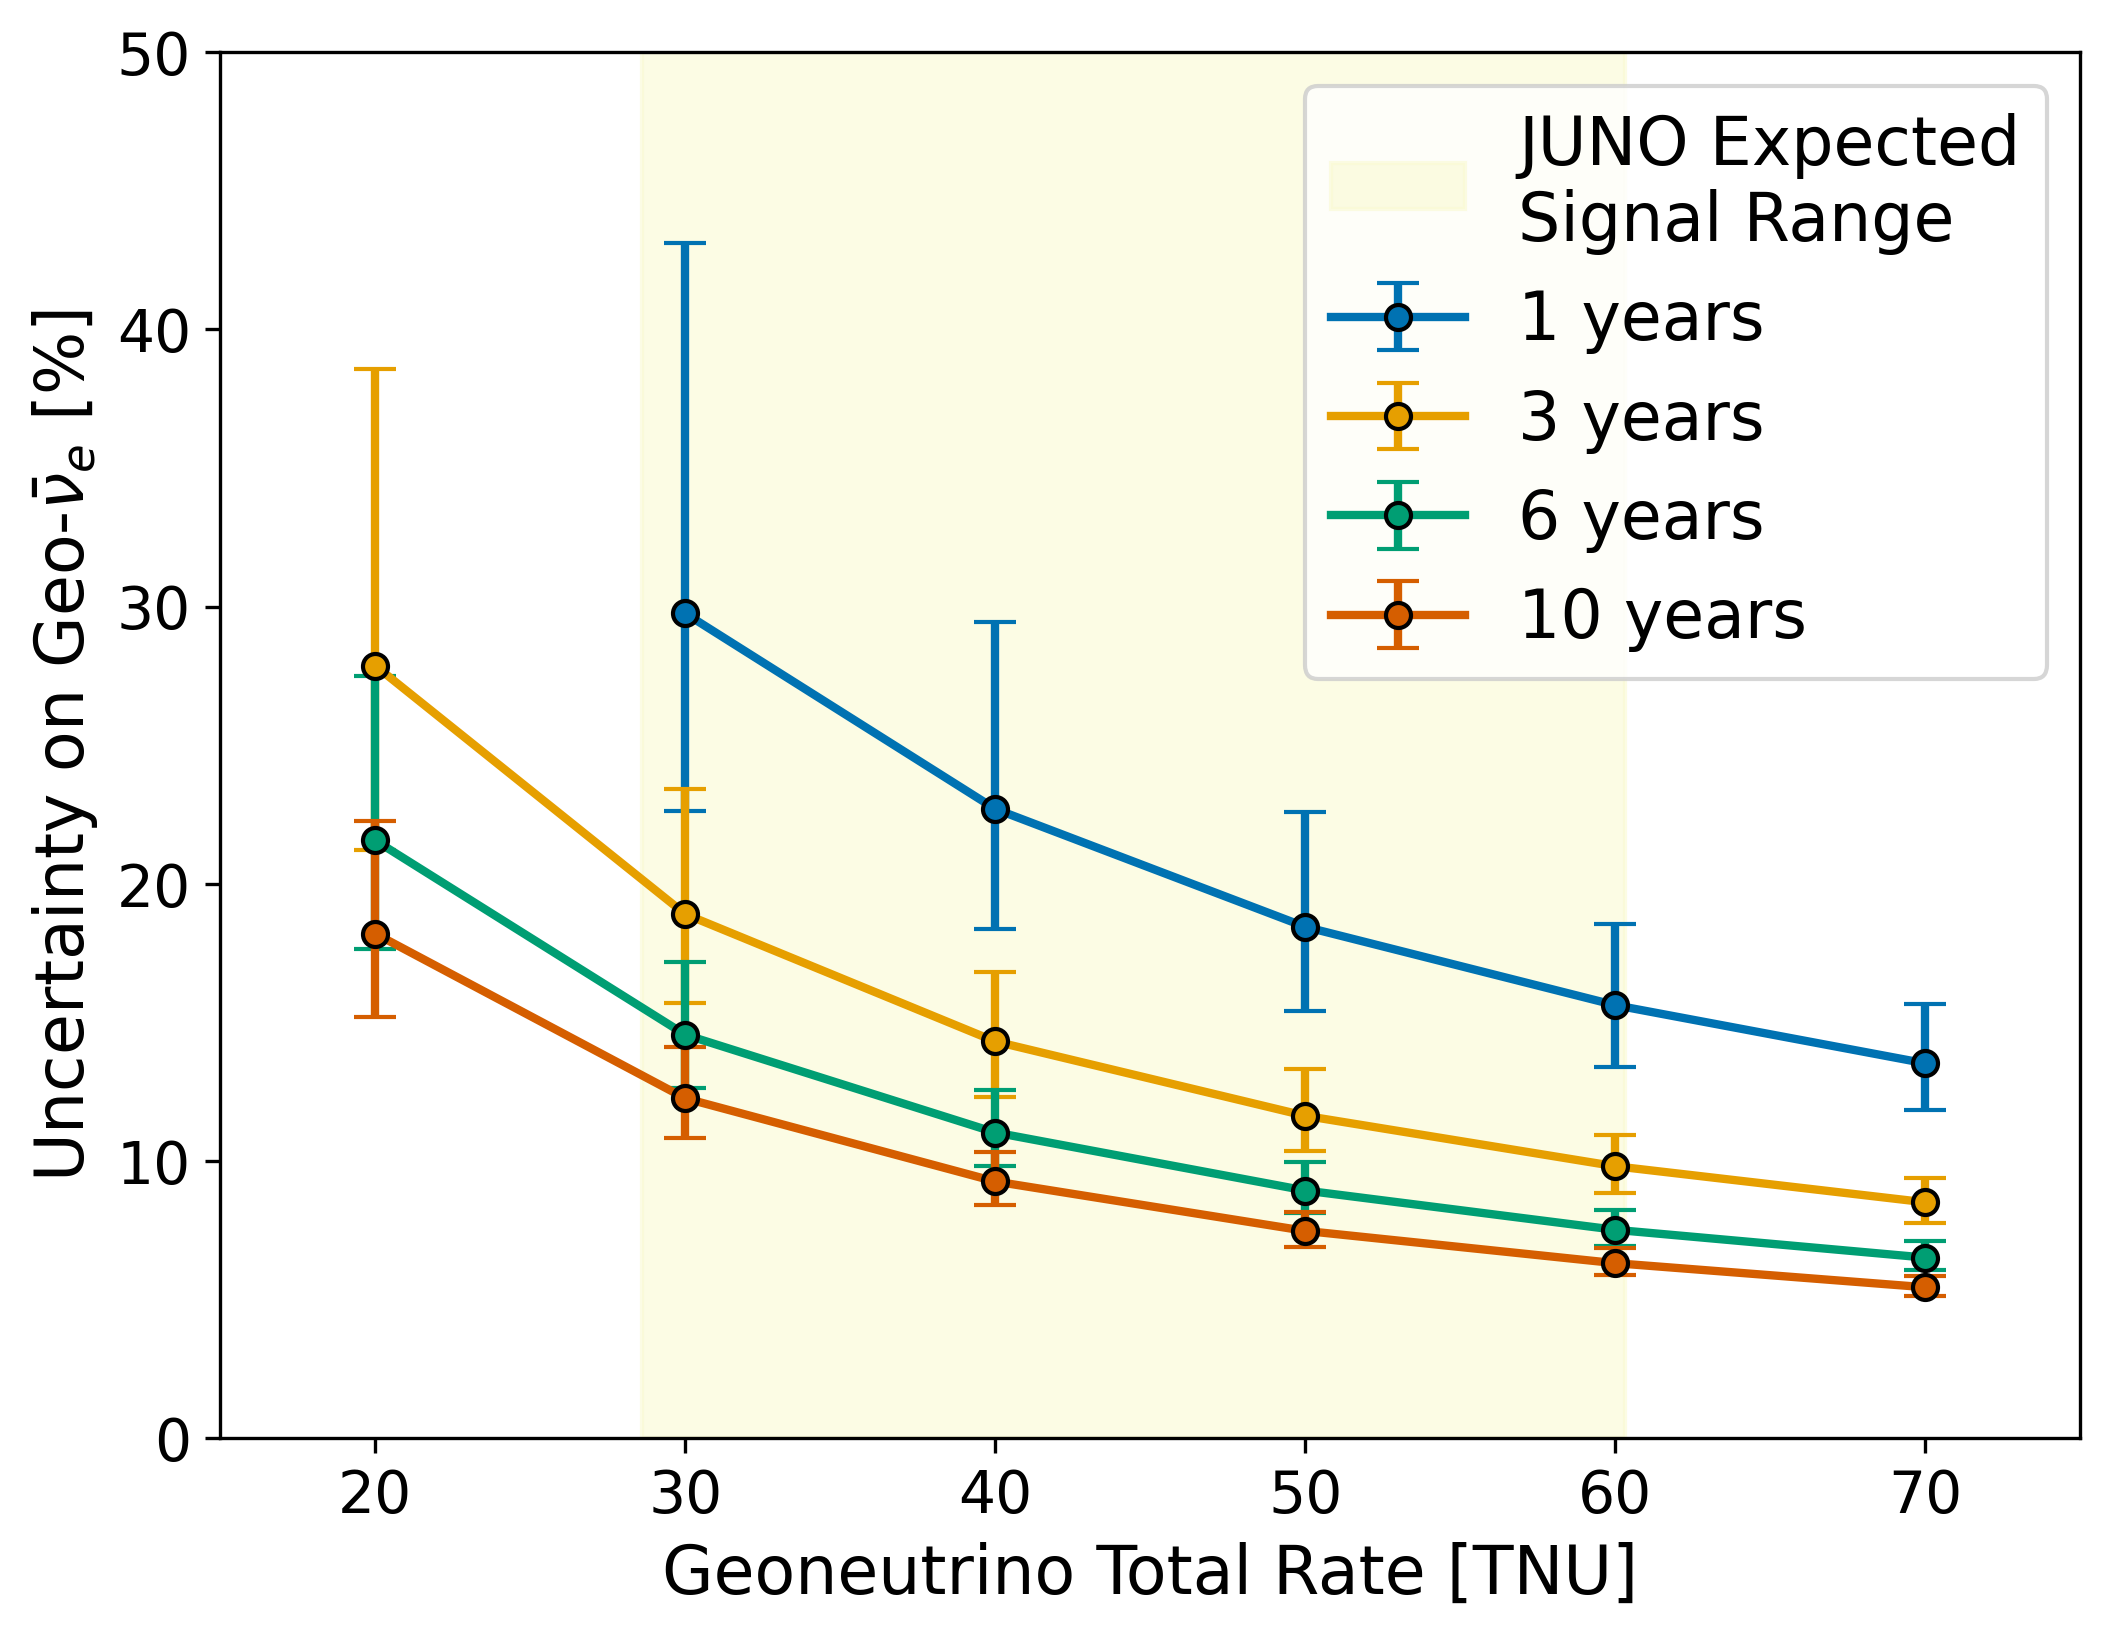
\includegraphics[width=0.9\linewidth]{Img/ScanGeo.png}
\bicaption[JUNO 对地球中微子总信号的预期测量精度]{JUNO 对地球中微子总信号的预期测量精度。图中给出了在假设 Th/U 比为球粒陨石比例条件下，JUNO 对地球中微子总信号（单位：TNU）的预期相对不确定度随总信号强度变化关系。蓝色、橙色、绿色和红色曲线分别对应 1 年、3 年、6 年和 10 年运行时间的灵敏度预期。纵轴表示对地球中微子总信号的相对不确定度（\%），横轴为地球中微子总事例率。黄色阴影区域表示不同 BSE（Bulk Silicate Earth）模型及岩石圈贡献预测所给出的 $1\sigma$ 信号区间。结果表明，随着运行时间增加，统计不确定度显著降低，在 10 年运行条件下可实现约 $5\%$--$7\%$ 量级的测量精度，从而对地球内部放射性元素分布模型形成重要约束。图片来自文献\citep{Li2026Prospects}}{Expected JUNO sensitivity to the total geoneutrino signal. The figure shows the projected relative uncertainty on the total geoneutrino signal (in TNU), assuming a fixed chondritic Th/U ratio, as a function of the total geoneutrino rate. The blue, orange, green, and red curves correspond to exposures of 1, 3, 6, and 10 years, respectively. The vertical yellow shaded region indicates the $1\sigma$ range of predicted signals from various Bulk Silicate Earth (BSE) models, including different assumptions for the lithospheric contribution. The results demonstrate that the measurement precision improves significantly with increased exposure, reaching approximately $5\%$--$7\%$ uncertainty after 10 years of operation, enabling strong constraints on Earth's radiogenic heat production models.Taken from Ref\citep{Li2026Prospects}}
\label{fig:geo_nu}
\end{figure}

如图~\ref{fig:geo_nu} 所示，随着运行时间的增加，JUNO 对地球中微子总信号的测量不确定度将显著降低，在 10 年运行条件下有望达到约 $5\%$ 量级的精度，从而有效区分不同 BSE 模型并约束地球内部放射性元素的分布。

\section{论文内容与结构}

本文围绕反应堆中微子振荡测量中的若干关键科学问题展开研究。针对低统计量条件下拟合偏差、联合分析中的模型依赖问题、振荡参数简并以及置信区间覆盖失效等现象，系统研究了合理的能谱分 bin 策略与Feldman-Cousins方法，并在此基础上提出了高性能的前向折叠反应堆中微子能谱计算与拟合框架，对基于大量 toy Monte Carlo 的分析流程进行了加速优化，以保证在有限算力条件下研究工作的可行性与精确性。

全文结构安排如下：

\textbf{第一章 引言}\\
本章首先回顾中微子的发现与基本物理性质，介绍中微子在标准模型中的地位及其可能的新物理含义，并系统梳理中微子振荡理论的基本框架。随后介绍江门中微子实验（JUNO）的探测结构、关键参数与主要物理目标，包括反应堆中微子、大气中微子、太阳中微子、超新星中微子以及地球中微子的探测研究，最后给出全文结构概述。

\textbf{第二章 中微子振荡分析方法（Oscillation Analysis Methods）}\\
本章系统介绍反应堆中微子的探测原理与能谱预测方法，包括核反应堆反中微子通量计算、沉积能量谱与重建能量谱构建，以及统计拟合方法的基本框架,同时介绍了前向折叠反应堆中微子拟合框架的能谱生成张量化表示。重点讨论低统计量条件下统计假设的适用性问题，分析 Wilks 定理的适用范围与局限性，并为后续引入 Feldman–Cousins 方法奠定理论基础。

\textbf{第三章 反应堆拟合程序的加速（Acceleration Strategies）}\\
由于分 bin 策略优化与 Feldman–Cousins 覆盖性研究均依赖海量 toy MC 实验，本章围绕拟合算法的性能优化展开研究。首先分析问题规模与性能瓶颈，随后从缓存技术、微分截面矩阵稀疏存储方式以及响应矩阵分块计算优化等方面实现算法加速，并对不同 bin 设置下的耗时影响进行系统测试，为大规模伪实验研究提供计算保障。

\textbf{第四章 JUNO 实验能谱分 bin 策略研究}\\
本章针对低统计量条件下高斯近似失效的问题，研究重建能谱的合理分 bin 策略，量化分 bin 选择对振荡参数偏差与精度的影响。进一步讨论 JUNO 与大亚湾（Daya Bay）联合分析中，由于两实验能量分辨率差异导致的 Wiggle 结构问题，指出若分 bin 过细可能超过 Daya Bay 实验约束能力，从而引入模型依赖系统误差。本章通过 Toy MC 系统研究不同分 bin 方案对结果稳定性与精度的影响，并提出合理优化方案。

\textbf{第五章 Feldman–Cousins 方法详述}\\
针对低统计量下振荡参数（特别是 $\Delta m^2_{31}$）存在简并、多极小值及不连续置信区间的问题，本章系统介绍 Feldman–Cousins 方法的基本思想与实现流程。通过大量 toy MC 实验研究 Wilks 近似的失效情况，验证 Feldman–Cousins 方法的覆盖性质，并分析临界值对扫描区间与参数空间的依赖性，确保置信区间具有正确的统计覆盖率。

\textbf{第六章 总结与展望}\\
本章对全文的研究工作进行系统总结，并对未来方向进行展望。总结部分回顾了基于张量化思想构建的高性能前向折叠反应堆中微子能谱计算与拟合框架、针对低统计量条件下重建能谱分 bin 与 JUNO--大亚湾联合分析中反应堆能谱分段（segment）策略的系统研究、以及基于 Feldman--Cousins 方法的频率学覆盖性检验三项主要成果，并阐述其对 JUNO 首篇物理结果论文所采用的统计方法与分段方案的实际贡献。展望部分讨论 JUNO 随统计量累积后 $\Delta m^2_{31}$ 精确测量所面临的非渐近统计挑战、JUNO 与近点高分辨率探测器 TAO 联合分析对实现近模型独立测量的关键作用，以及在质量序判定、无中微子双贝塔衰变（$0\nu\beta\beta$）与 CP 破坏相位测定等国际中微子物理前沿方向上的研究前景。

\section{本章小结}

本章系统回顾了中微子物理的研究脉络与基本物理性质：从 $\beta$ 衰变能量连续谱之谜与泡利中微子假说出发，梳理了三代中微子的相继发现以及宇称破缺、二分量中微子理论与中微子左旋性的确立；进而讨论了中微子在标准模型中的地位，阐述了为解释非零中微子质量而引入的跷跷板机制等新物理图像，并系统介绍了 PMNS 混合矩阵、真空三味振荡概率以及 MSW 物质效应等振荡理论要素，给出了后续分析所依赖的反应堆反中微子存活概率表达式。

本章还介绍了江门中微子实验（JUNO）的探测器结构与关键性能指标——包括 20\,kt 液体闪烁体中心探测器、水切伦科夫屏蔽以及 20 英寸与 3 英寸 PMT 构成的双量能器系统，达到约 3\% @ 1\,MeV 的能量分辨率——并概述了 JUNO 对反应堆中微子、大气中微子、太阳中微子、超新星中微子和地球中微子等多种中微子源的探测能力及主要物理目标。2025 年底发布的 JUNO 首篇物理结果已将太阳振荡参数 $\sin^2\theta_{12}$ 与 $\Delta m^2_{21}$ 的测量精度相对全球既有结果提升约 1.6 倍，标志着中微子物理由"发现时代"进入"高精度测量时代"。这些物理背景与实验概况为后续章节围绕反应堆中微子振荡测量所展开的能谱预测框架构建、分 bin 与分段策略研究以及 Feldman--Cousins 覆盖性检验等方法学工作奠定了物理基础。
